%%%%%%%%%%%%%%%%%%%%%%%%
%
% $Autor: Hemanth Jadiswami Prabhakaran $
% $Datum: 2025-06-30 11:18:21Z $
% $Pfad: GitHub/BA25-01-Time-Series/Manual/Chapters/en/01IntroductionAndMainFunction.tex $
% $Version: 1 $
%
% $Project: BA25-Time-Series $
%
%%%%%%%%%%%%%%%%%%%%%%%%



\chapter{Introduction and Main Function}

\section{Overview}

The Walmart Sales Forecasting System is a comprehensive two-application solution developed as part of a Master's Business Analytics course project. This system demonstrates advanced time series forecasting capabilities using state-of-the-art machine learning algorithms to predict weekly sales changes for retail environments.

The system architecture consists of two complementary applications designed to provide a complete forecasting workflow from model development to production predictions.

\begin{figure}[H]
    \centering
    \begin{tikzpicture}[
	node distance=3cm and 4cm,
	block/.style={rectangle, draw, fill=blue!20, text width=4cm, text centered, rounded corners, minimum height=1.5cm},
	data/.style={rectangle, draw, fill=orange!20, text width=4cm, text centered, rounded corners, minimum height=1.5cm},
	model/.style={rectangle, draw, fill=yellow!20, text width=4cm, text centered, rounded corners, minimum height=1.5cm},
	output/.style={rectangle, draw, fill=purple!20, text width=4cm, text centered, rounded corners, minimum height=1.5cm},
	user/.style={ellipse, draw, fill=red!20, text width=3cm, text centered, minimum height=1cm},
	arrow/.style={thick,->,>=stealth}
	]
	
	% Title
	\node at (0,10) {\Large\textbf{Walmart Sales Forecasting System Architecture}};
	
	% User
	\node[user] (user) at (0,8.5) {Users\\(Browser or Python)};
	
	% Data Sources
	\node[data] (data) at (0,6) {Data Sources\\train.csv\\features.csv\\stores.csv};
	
	% Training Apps
	\node[block] (cloud_train) at (-4,3) {Cloud Training App\\(Streamlit Cloud)};
	\node[block] (local_train) at (4,3) {Local Training App\\(localhost:8501)};
	
	% Model Storage
	\node[model] (models) at (0,0) {Model Storage\\ARIMA, Exp. Smoothing};
	
	% Prediction Apps
	\node[block] (cloud_pred) at (-4,-3) {Cloud Prediction App\\(Streamlit Cloud)};
	\node[block] (local_pred) at (4,-3) {Local Prediction App\\(localhost:8502)};
	
	% Output
	\node[output] (output) at (0,-6) {Forecast Output\\4-week predictions\\CSV/JSON, Visuals};
	
	% Arrows
	\draw[arrow] (user) -- (data);
	\draw[arrow] (data) -- (cloud_train);
	\draw[arrow] (data) -- (local_train);
	\draw[arrow] (cloud_train) -- (models);
	\draw[arrow] (local_train) -- (models);
	\draw[arrow] (models) -- (cloud_pred);
	\draw[arrow] (models) -- (local_pred);
	\draw[arrow] (cloud_pred) -- (output);
	\draw[arrow] (local_pred) -- (output);
	
\end{tikzpicture}
    \caption{Walmart Sales Forecasting System Architecture Overview}
    \label{fig:system_architecture}
\end{figure}

\section{Primary Capabilities}

\subsection{Dual-Application Architecture}

The system operates through two specialized applications, each serving distinct functions in the forecasting pipeline:

\begin{enumerate}
    \item \textbf{Training Application}: Provides a user-friendly interface for developing and training new forecasting models
    \item \textbf{Prediction Application}: Delivers production-ready forecasting capabilities with pre-trained models
\end{enumerate}

\begin{figure}[H]
    \centering
  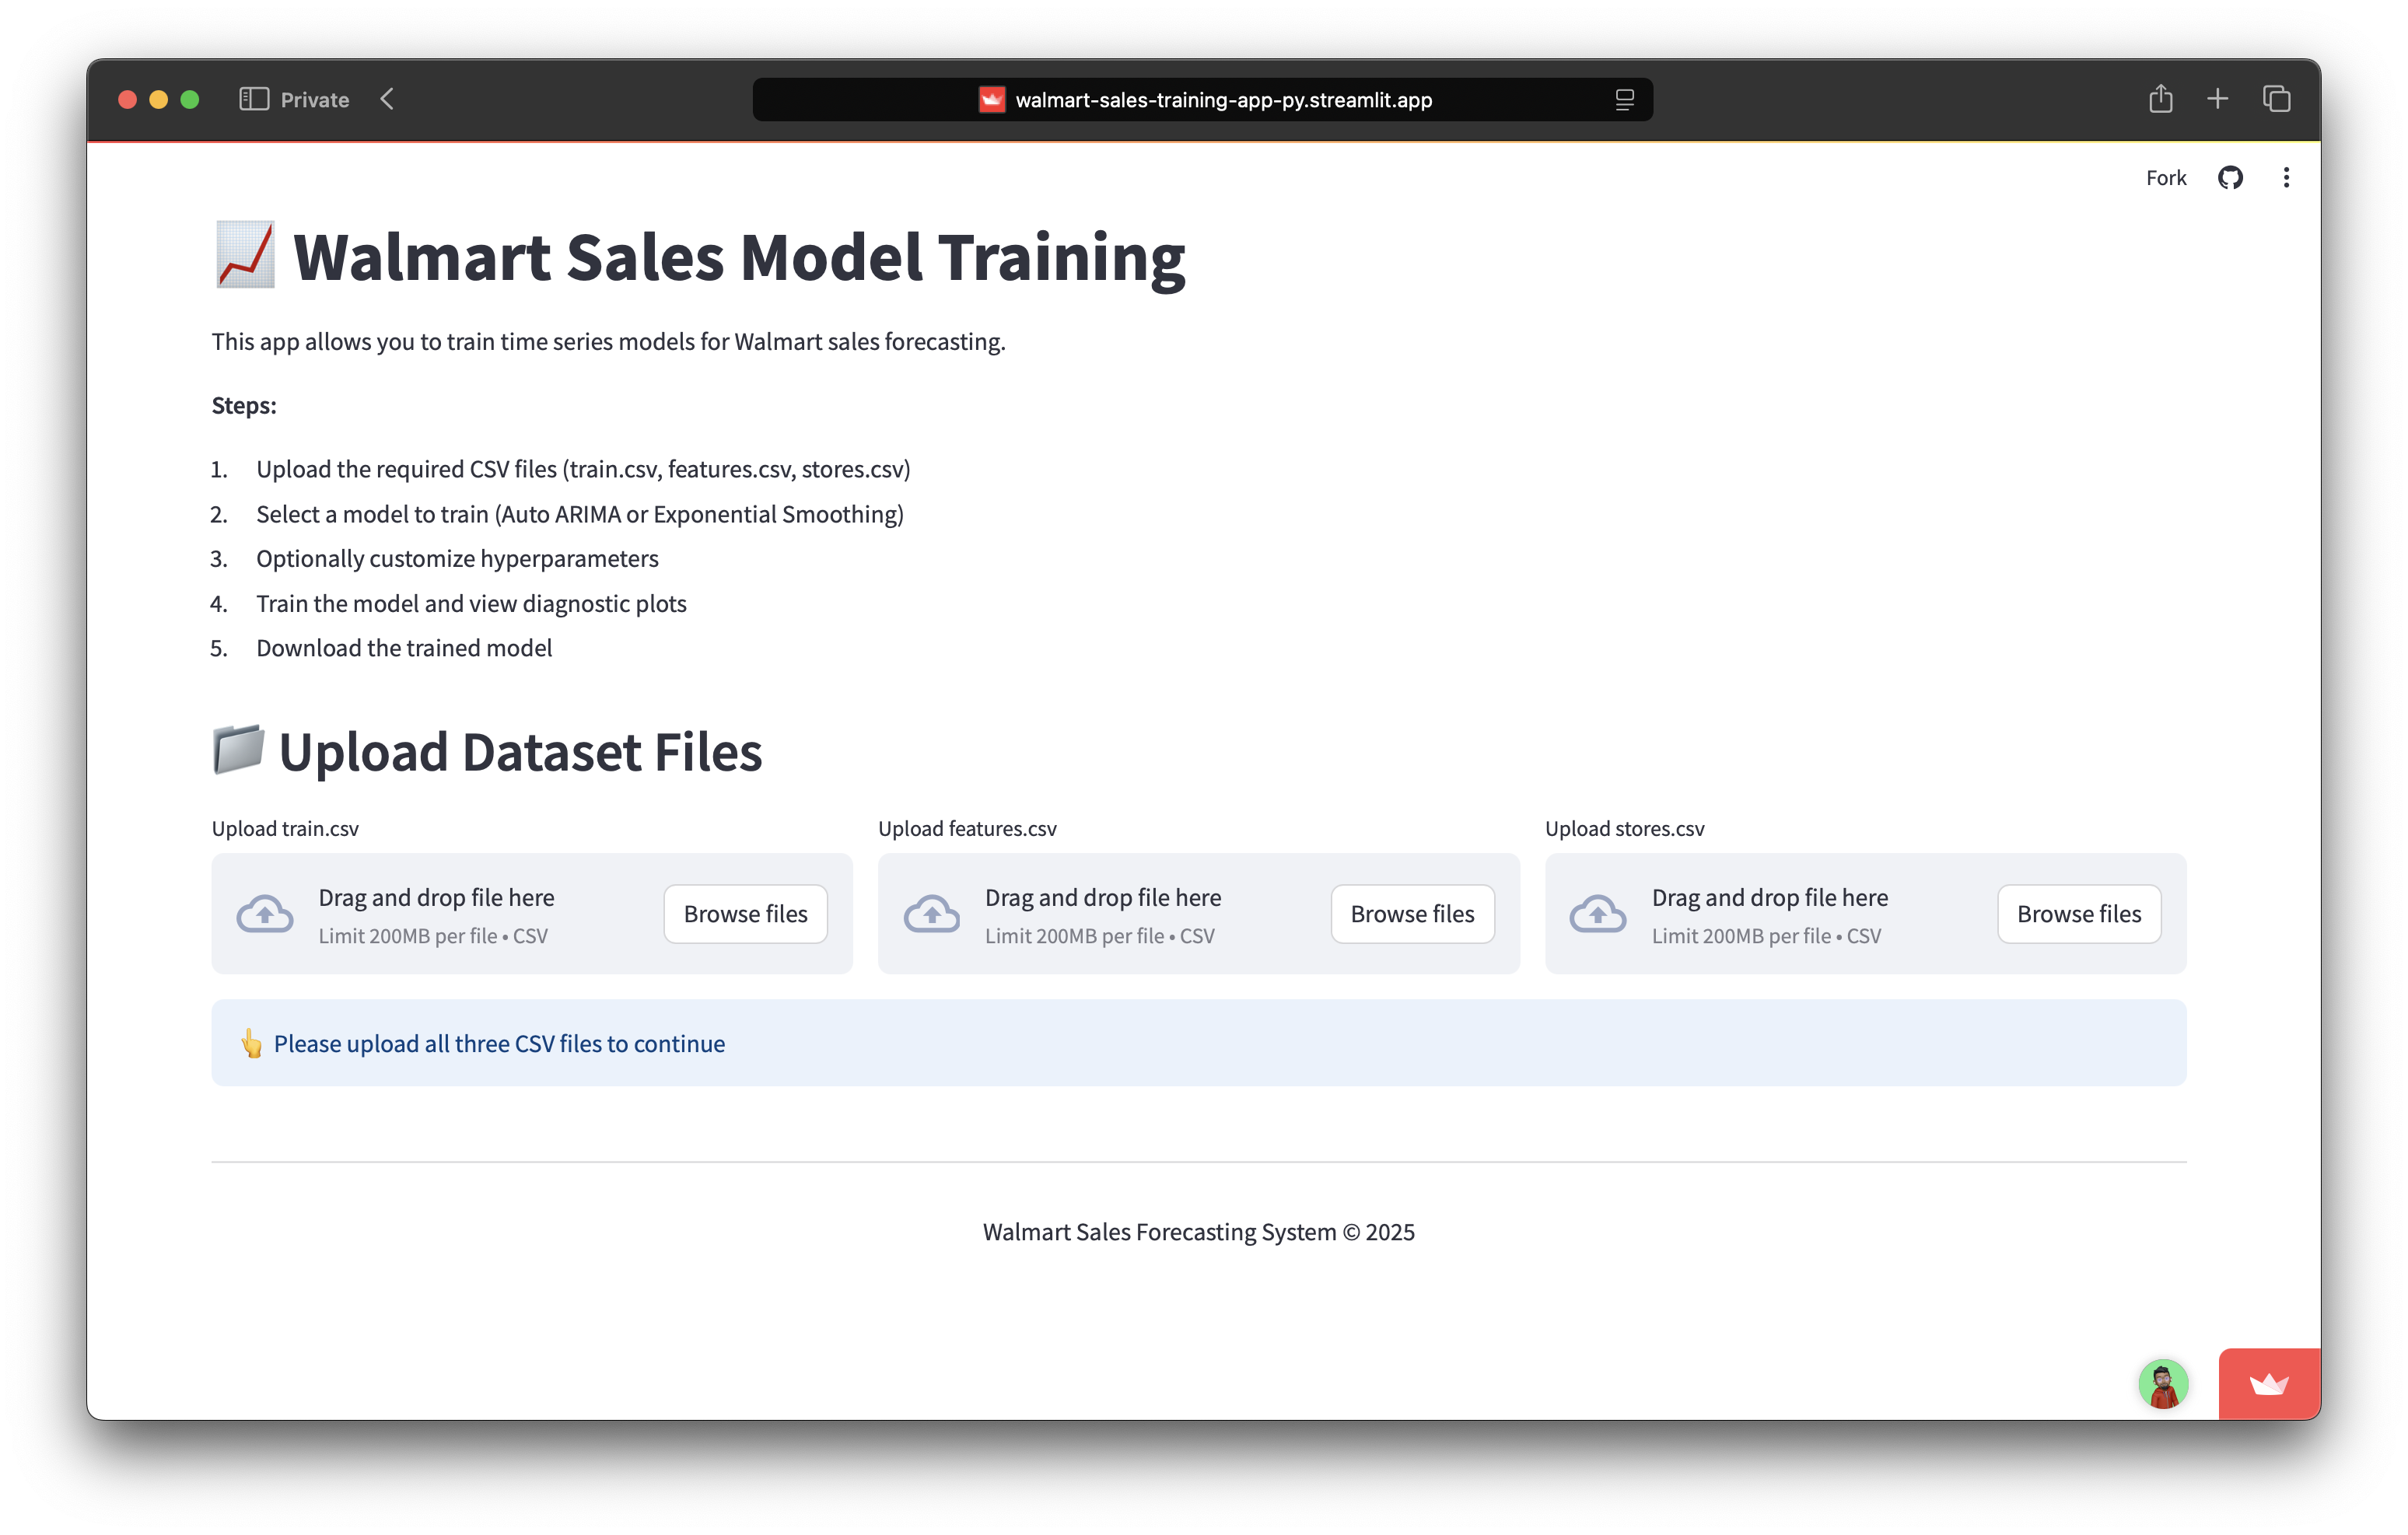
\includegraphics[width=0.9\textwidth]{Images/01IntroductionAndMainFunction/TrainingAppMainInterface.png}
  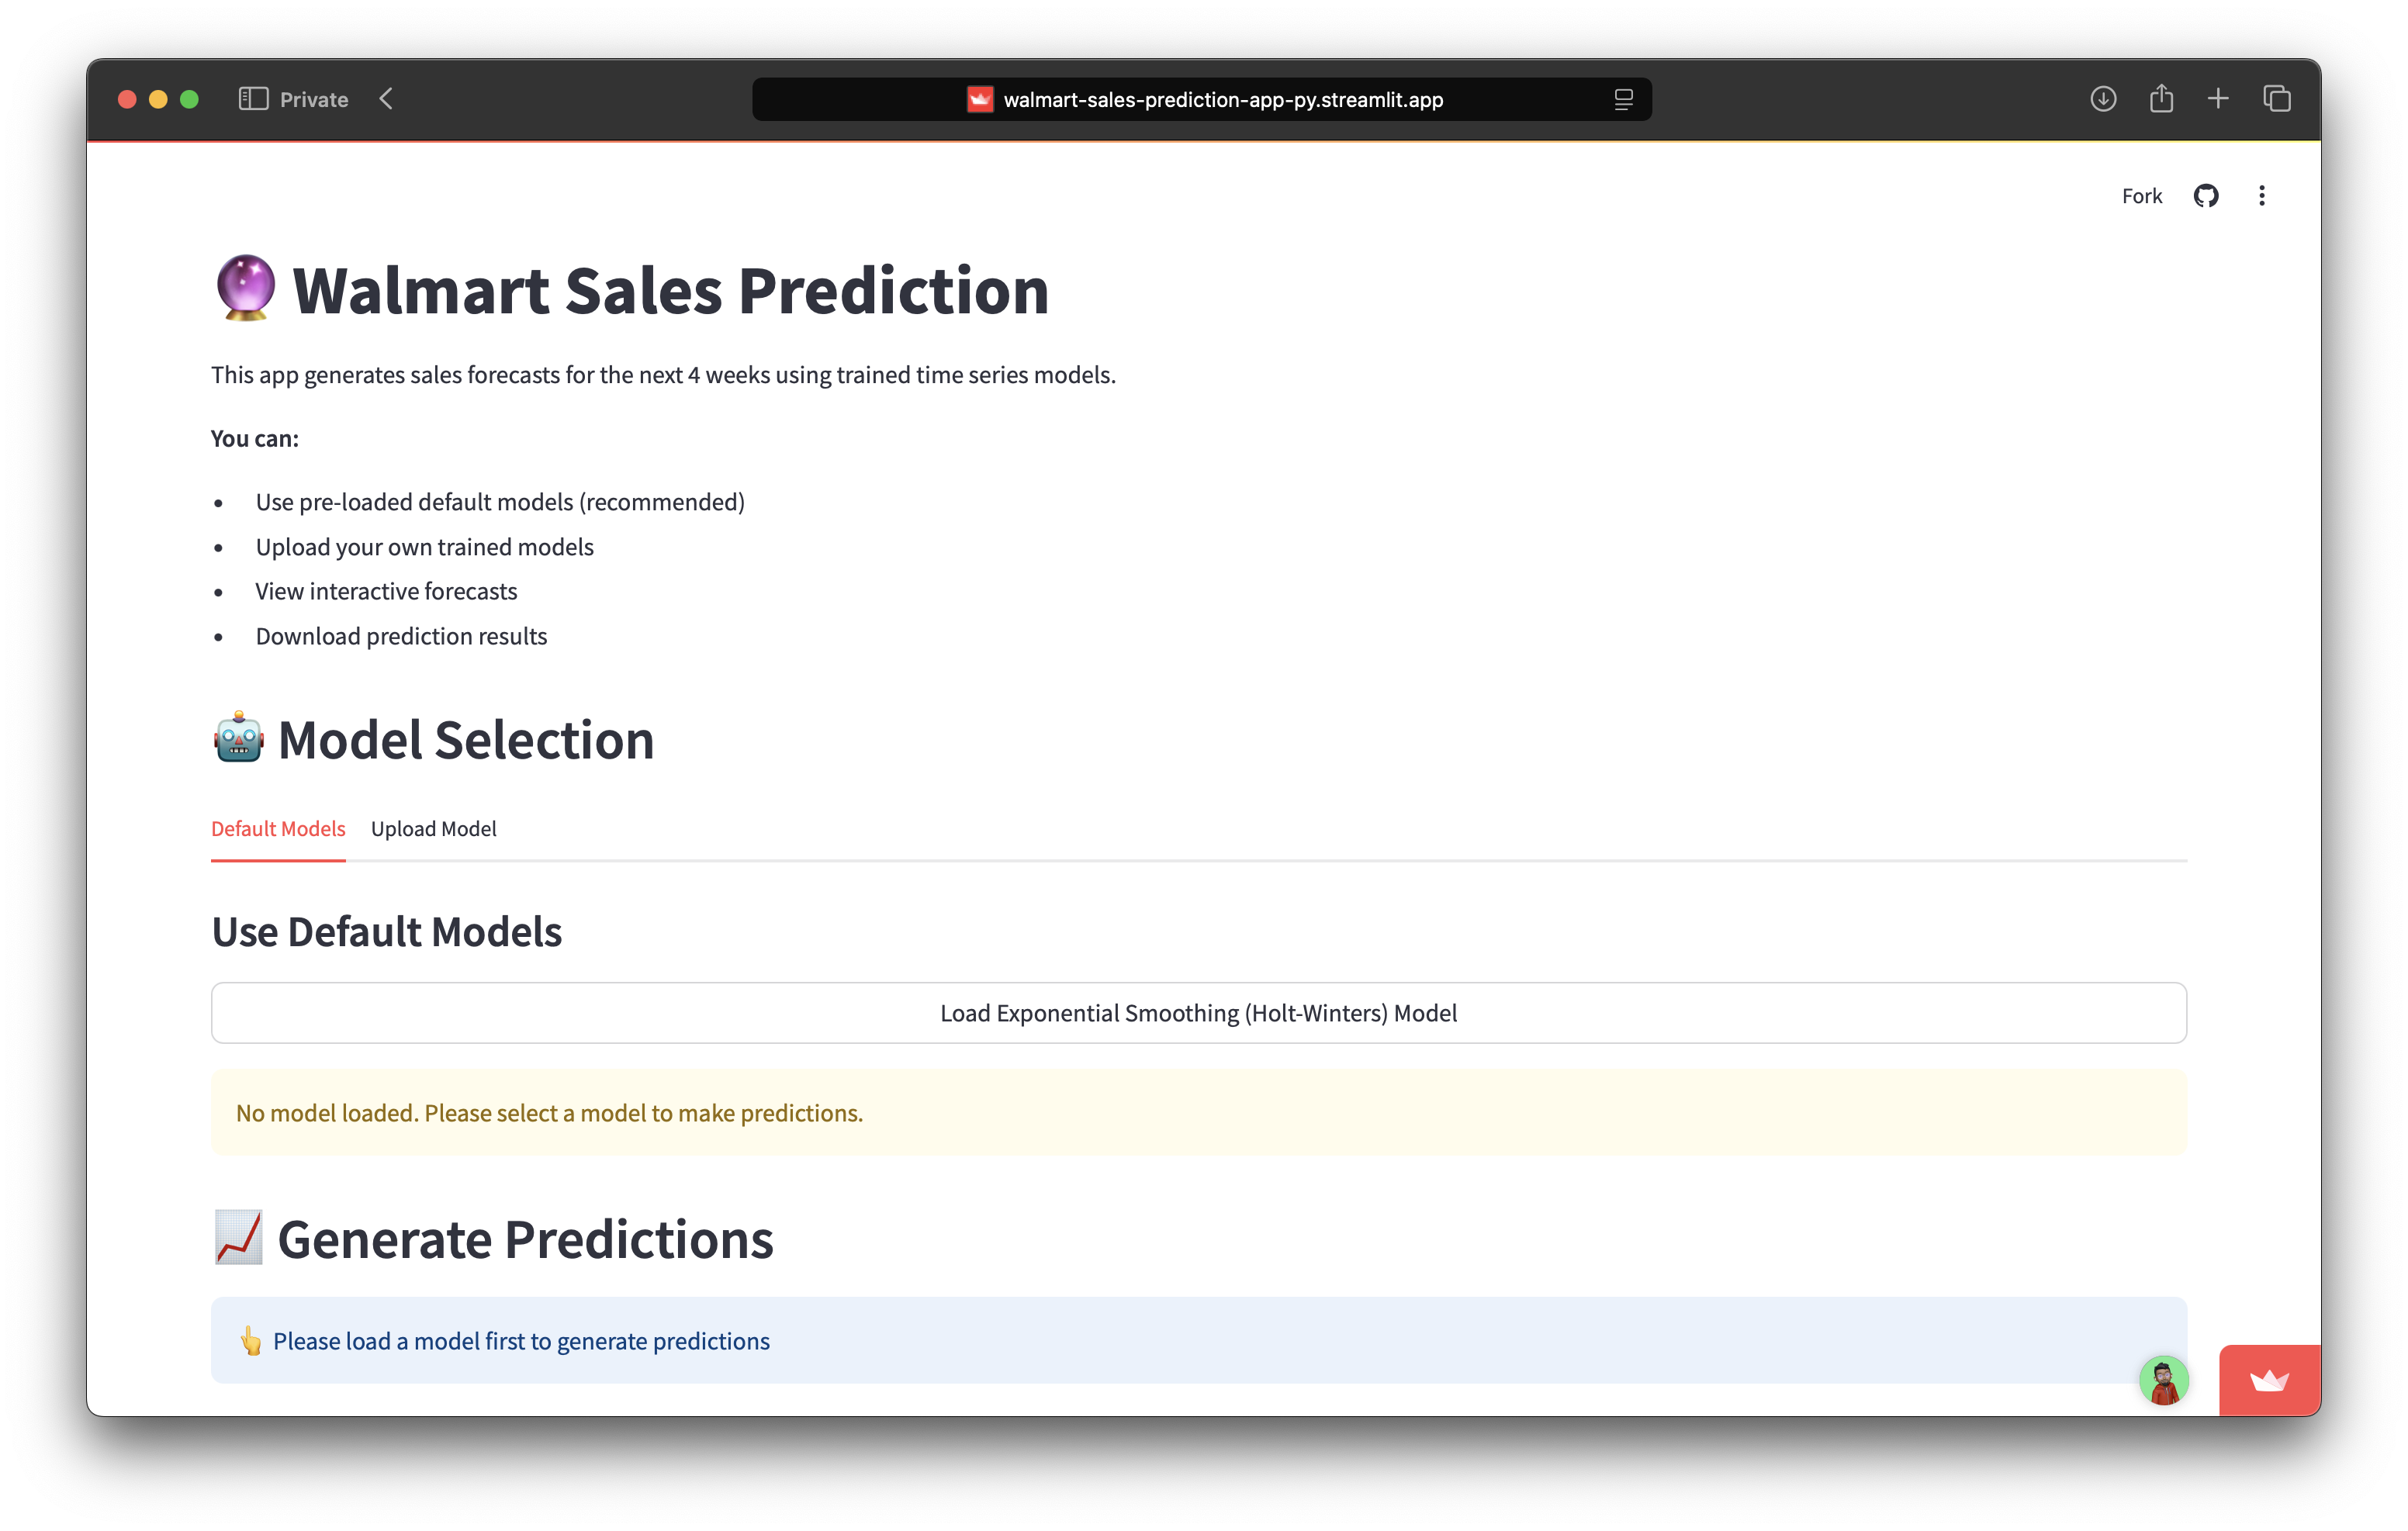
\includegraphics[width=0.9\textwidth]{Images/01IntroductionAndMainFunction/PredictionAppMainInterface.png}
    \caption{Dual-Application Interface Comparison}
    \label{fig:application_overview}
\end{figure}

\subsection{Advanced Time Series Modeling}

The system implements two sophisticated forecasting algorithms:

\begin{itemize}
    \item \textbf{Auto ARIMA}: Automated ARIMA model selection with seasonal components
    \item \textbf{Exponential Smoothing (Holt-Winters)}: Triple exponential smoothing with trend and seasonal components
\end{itemize}

\subsection{Flexible Deployment Options}

Both applications support multiple deployment scenarios:

\begin{itemize}
    \item \textbf{Cloud Access}: Immediate browser-based access via Streamlit Cloud
    \item \textbf{Local Installation}: Python 3.12 virtual environment setup for offline usage
\end{itemize}

\section{Core Functionality}

\subsection{Model Training Capabilities}

The Training Application provides comprehensive model development features:

\begin{itemize}
    \item \textbf{Data Upload}: Support for standard Walmart dataset format (train.csv, features.csv, stores.csv)
    \item \textbf{Automated Preprocessing}: Data cleaning, validation, and feature engineering
    \item \textbf{Hyperparameter Tuning}: Customizable model parameters for optimal performance
    \item \textbf{Performance Evaluation}: WMAE-based model assessment with visual diagnostics
    \item \textbf{Model Export}: Trained models saved in .pkl format for deployment
\end{itemize}

\begin{figure}[H]
    \centering
   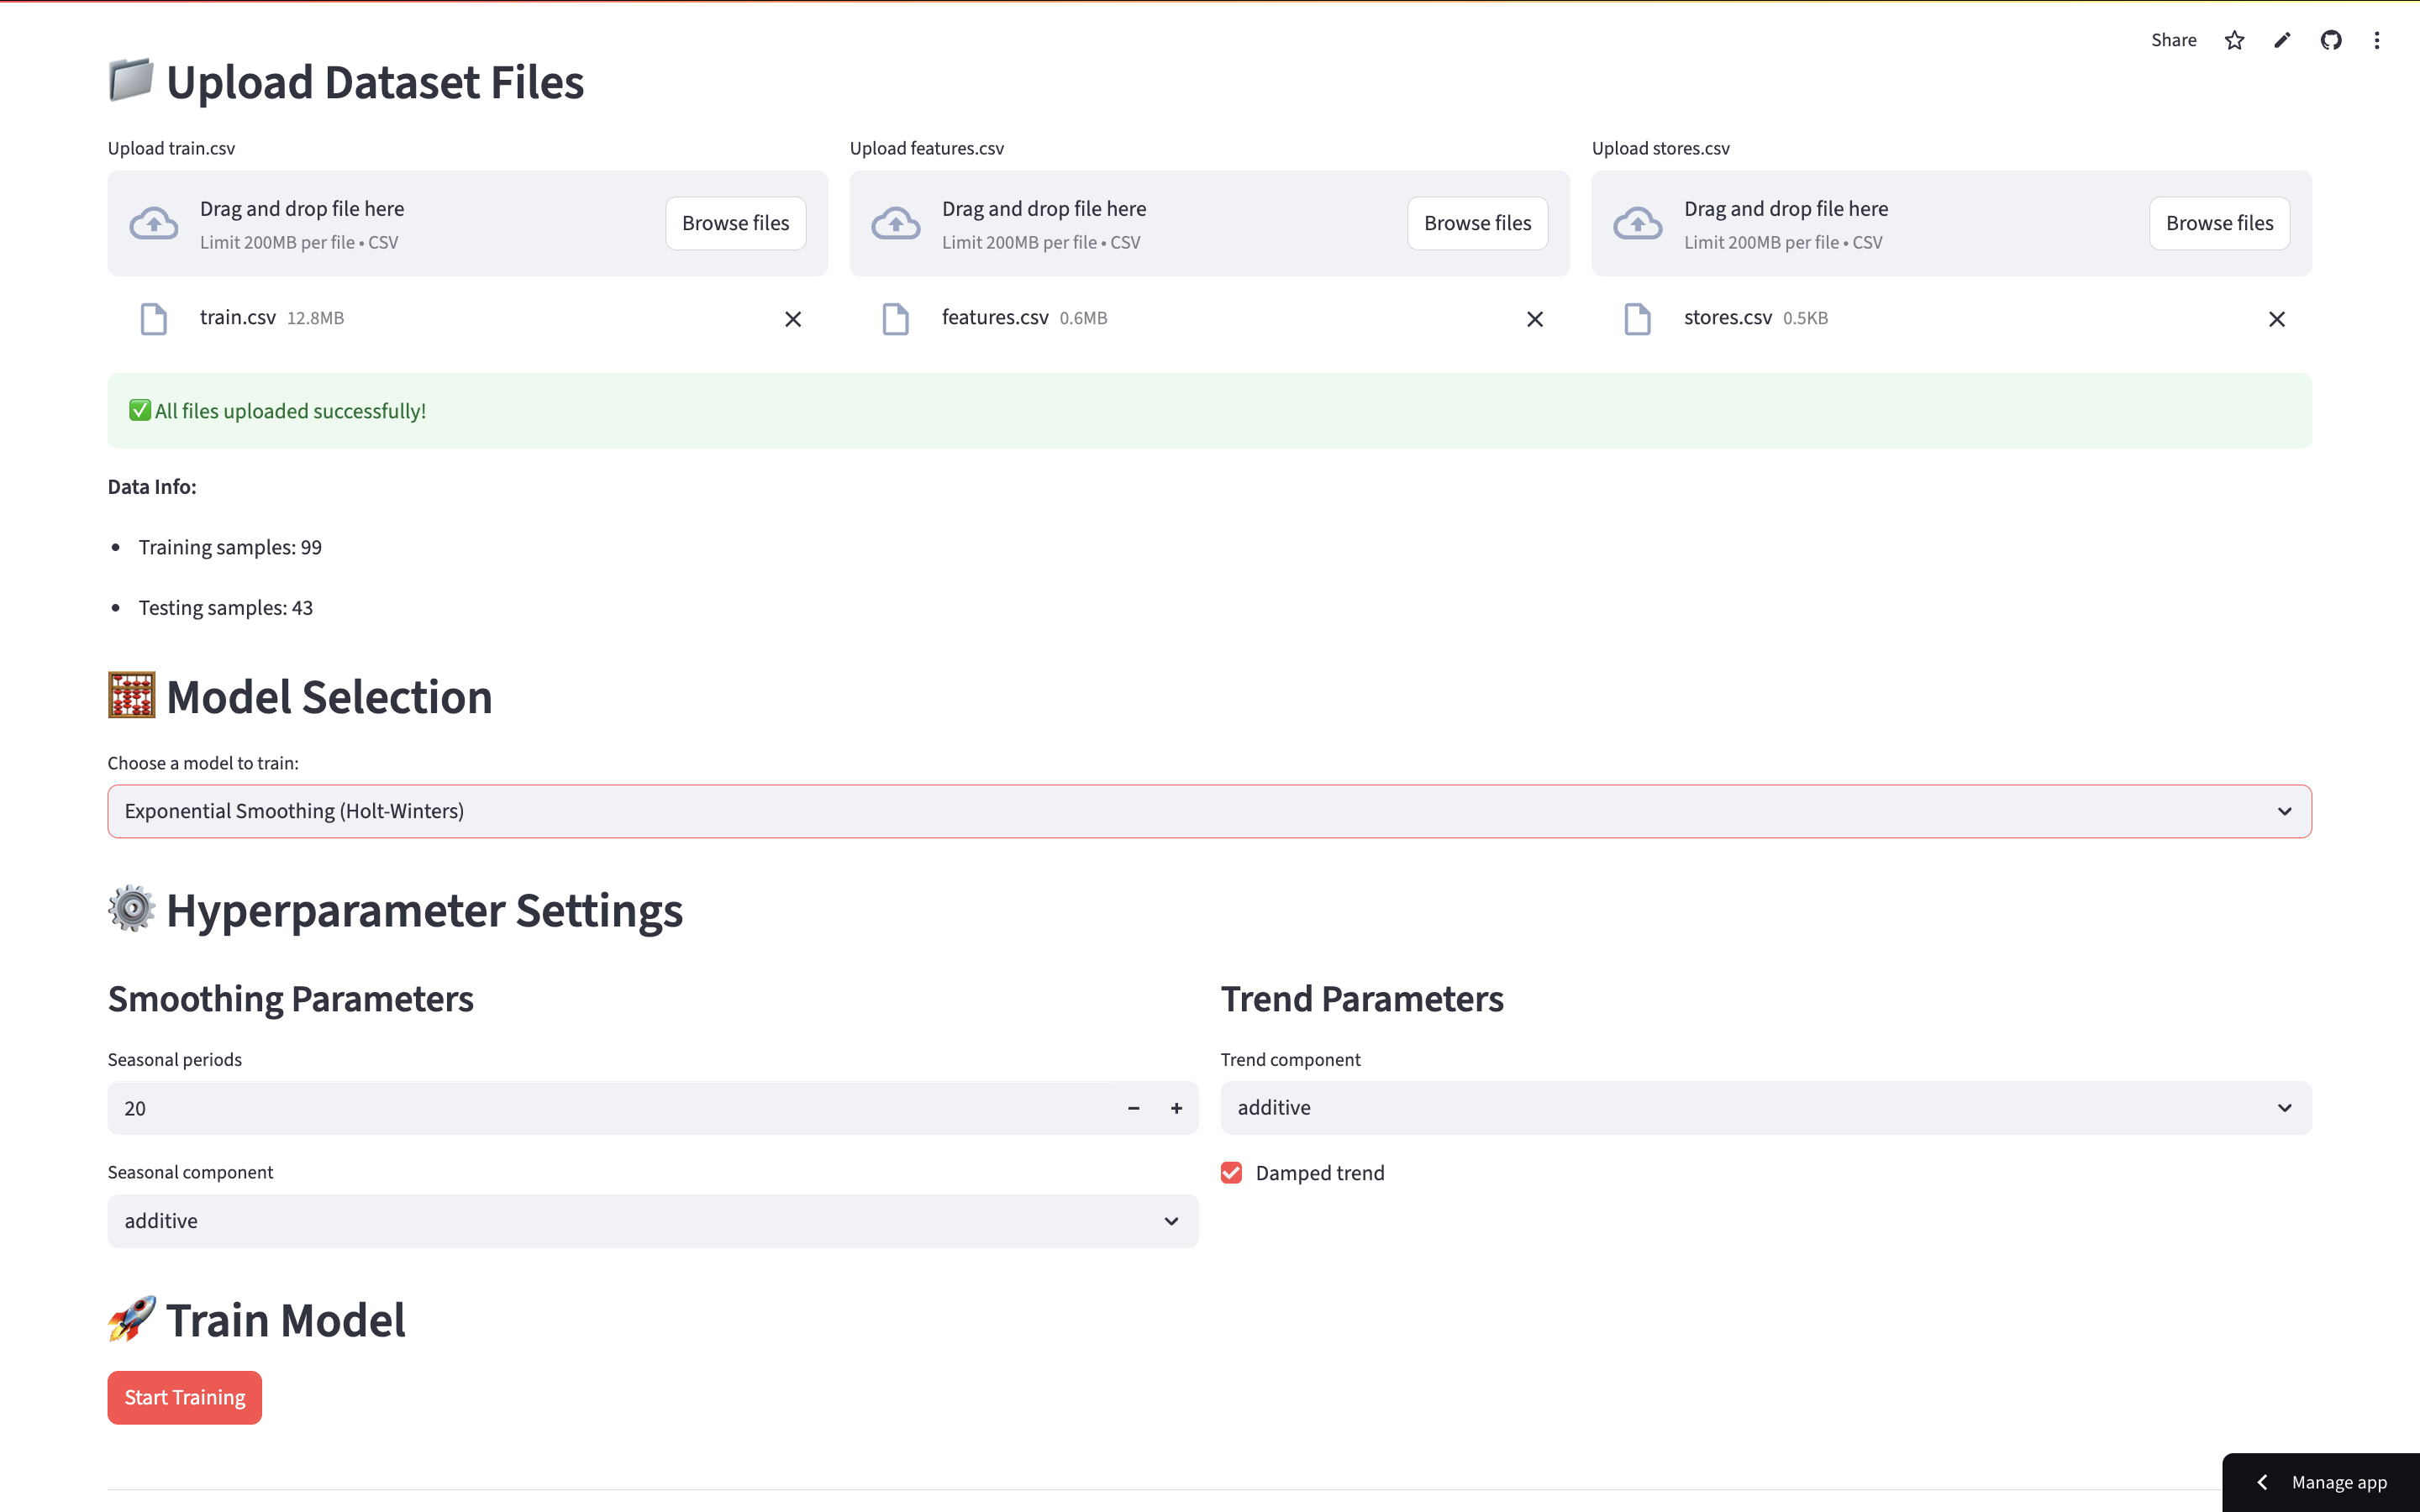
\includegraphics[width=0.9\textwidth]{Images/01IntroductionAndMainFunction/TrainingWorkflow.png}
    \caption{Model Training Workflow Interface}
    \label{fig:training_workflow}
\end{figure}

\subsection{Production Forecasting Features}

The Prediction Application offers robust forecasting capabilities:

\begin{itemize}
    \item \textbf{Pre-loaded Model}: High-performance Exponential Smoothing model (3.58\% WMAE)
    \item \textbf{Custom Model Support}: Upload and use personally trained models
    \item \textbf{4-Week Forecasting}: Generate week-over-week sales change predictions
    \item \textbf{Interactive Visualizations}: Dynamic charts with positive/negative change indicators
    \item \textbf{Export Capabilities}: Download results in CSV and JSON formats
\end{itemize}

\begin{figure}[H]
    \centering
    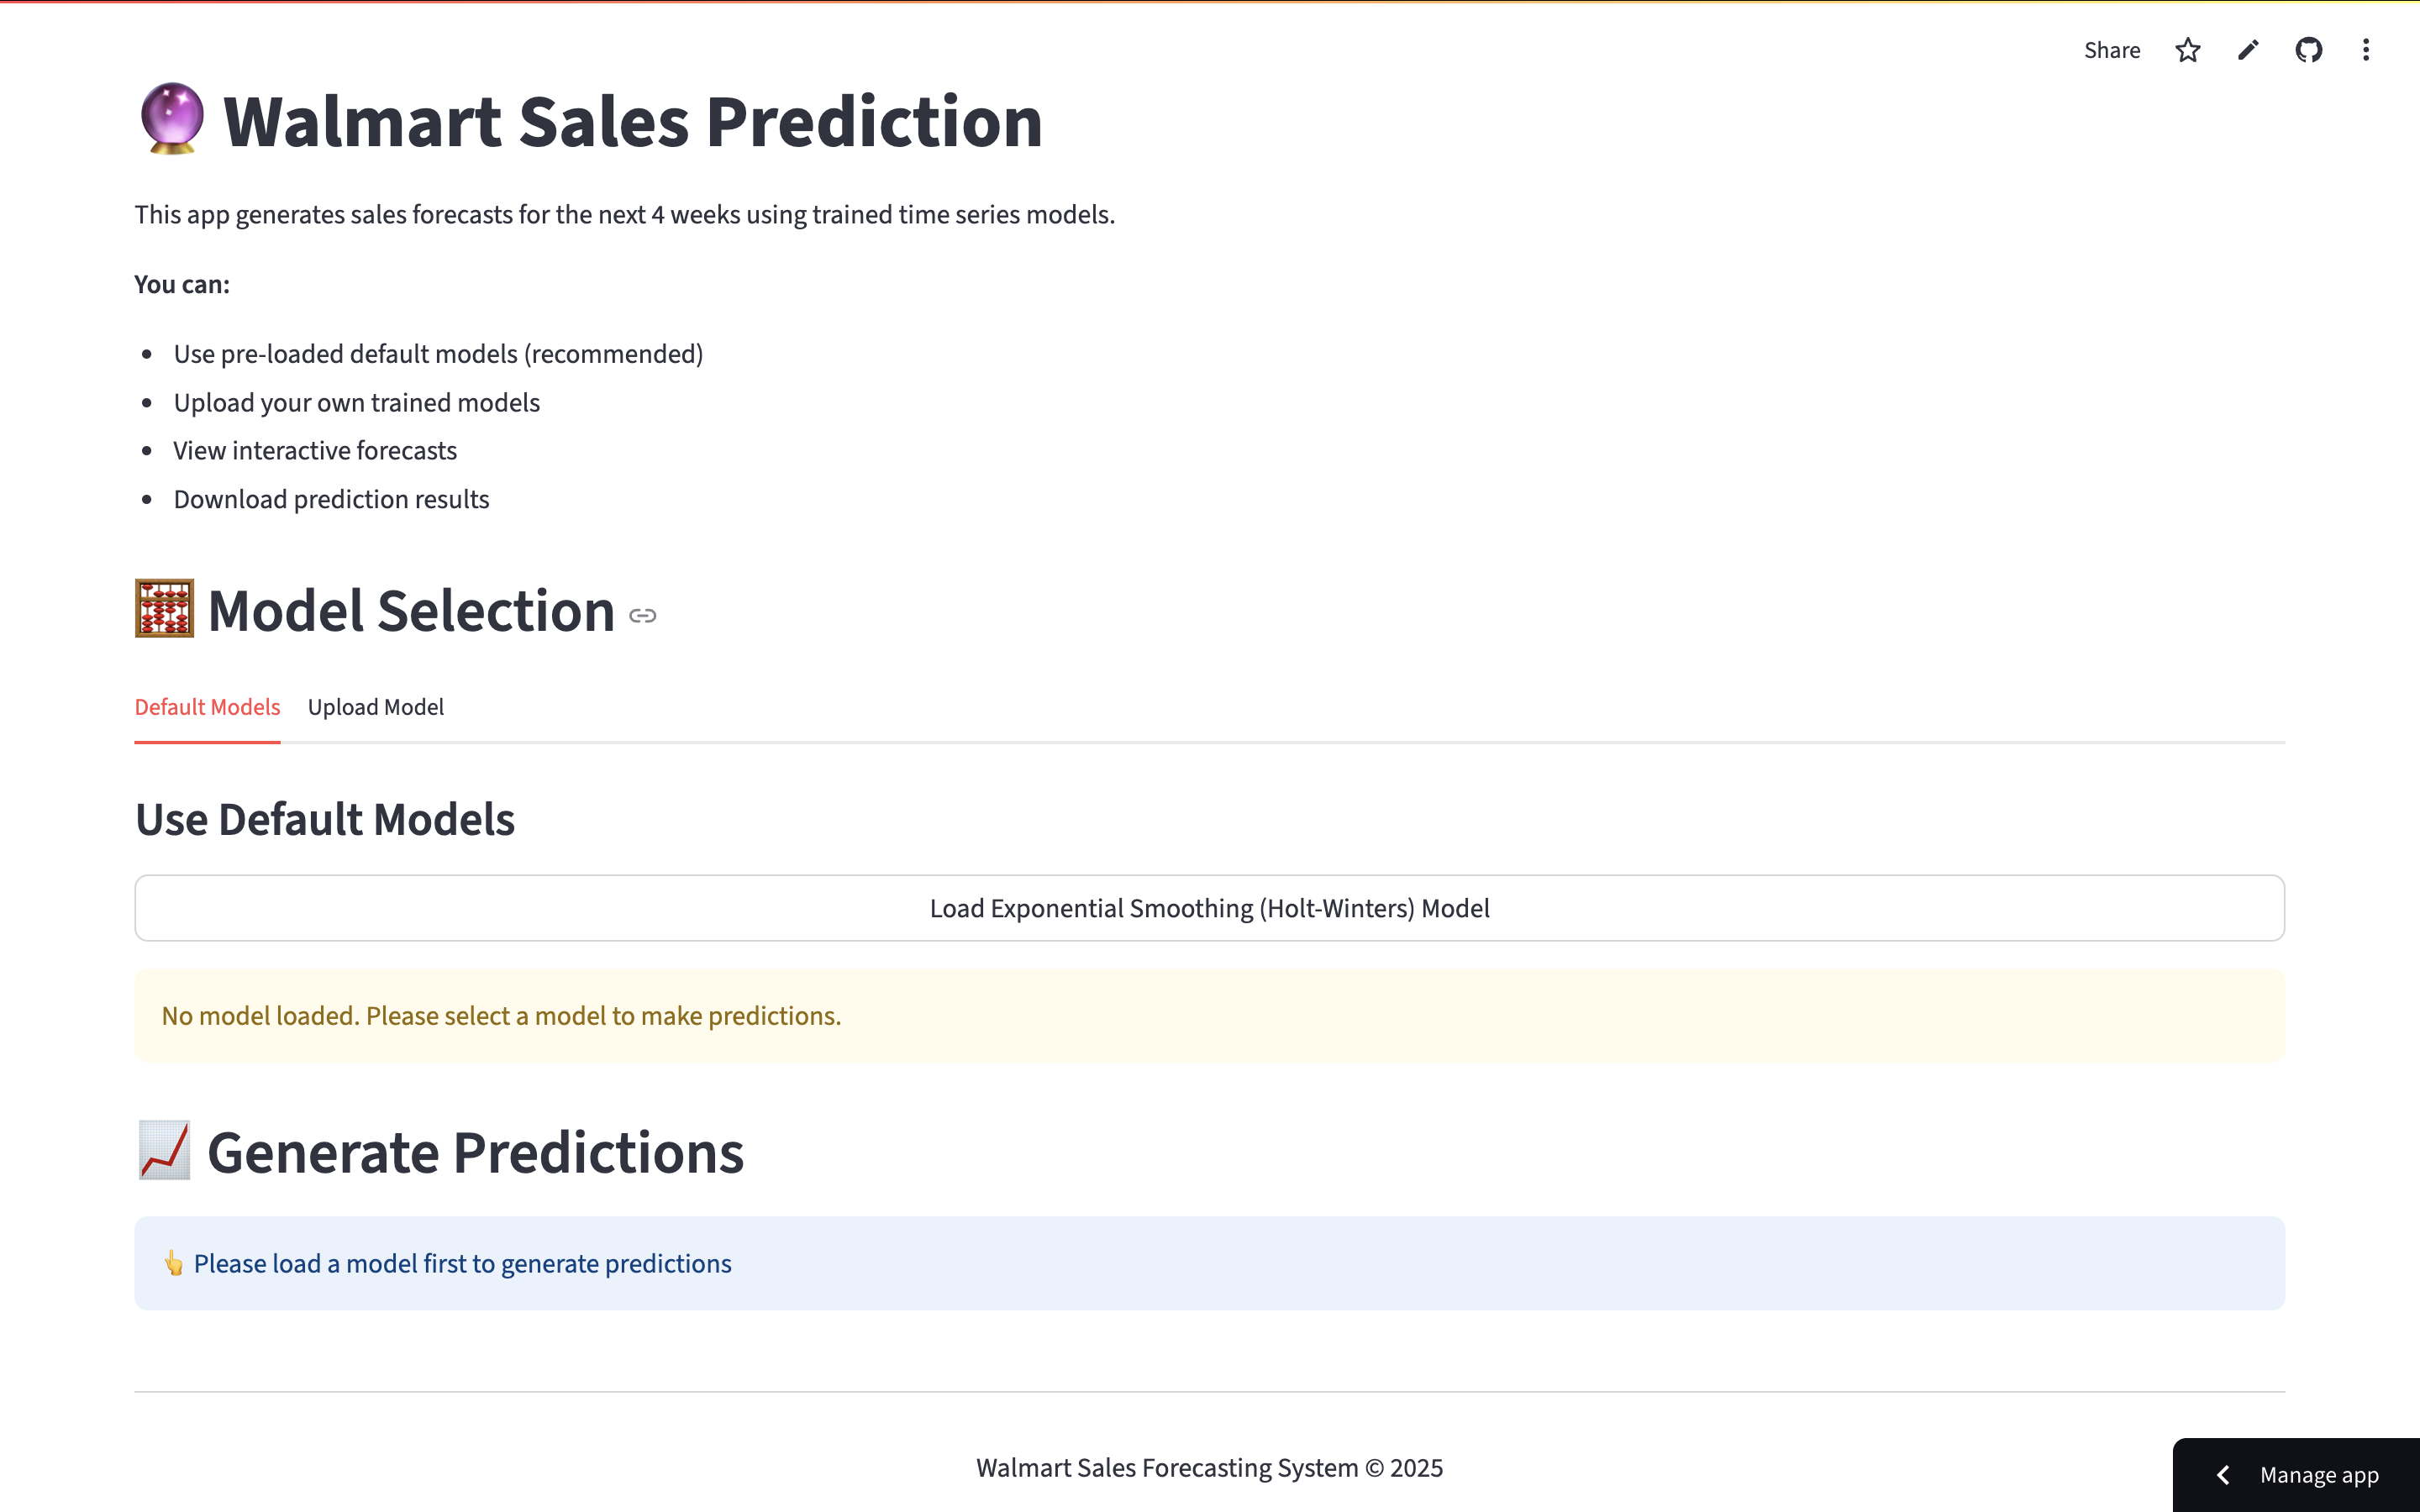
\includegraphics[width=0.9\textwidth]{Images/01IntroductionAndMainFunction/PredictionInterface.png}
    \caption{Prediction Application Main Interface}
    \label{fig:prediction_interface}
\end{figure}

\section{Key Performance Characteristics}

\subsection{Model Accuracy}

The default Exponential Smoothing (Holt-Winters) model demonstrates excellent performance:

\begin{itemize}
    \item \textbf{Normalized WMAE}: 3.58\% (Excellent category - less than 5\% error)
    \item \textbf{Absolute WMAE}: 923.12 (dollars in weekly sales change)
    \item \textbf{Prediction Horizon}: 4 weeks ahead
\end{itemize}

\subsection{Technical Specifications}

\begin{itemize}
    \item \textbf{Python Version}: 3.12 (exact version requirement)
    \item \textbf{Framework}: Streamlit for web interface
    \item \textbf{Model Format}: Joblib .pkl serialization
    \item \textbf{Data Format}: CSV input with specific schema requirements
\end{itemize}

\section{Target Applications}

This forecasting system is designed for multiple use cases:

\begin{itemize}
    \item \textbf{Academic Research}: Educational tool for time series analysis learning
    \item \textbf{Business Analytics}: Sales forecasting for retail planning
    \item \textbf{Model Development}: Platform for experimenting with forecasting algorithms
    \item \textbf{Production Deployment}: Operational forecasting for decision support
\end{itemize}

\section{Document Structure}

This user manual provides comprehensive guidance organized into nine core chapters:

\begin{enumerate}
    \item \textbf{Introduction and Main Function}: System overview and capabilities
    \item \textbf{Installation and Setup}: Local and cloud deployment procedures
    \item \textbf{First Steps Guide}: Initial usage walkthrough
    \item \textbf{GUI and User Interface}: Detailed interface documentation
    \item \textbf{Application Functions}: Complete feature coverage
    \item \textbf{System Specifications}: Technical requirements and data formats
    \item \textbf{Maintenance and Best Practices}: Operational guidance
    \item \textbf{Troubleshooting}: Problem resolution procedures
    \item \textbf{Help and Support}: Additional assistance resources
\end{enumerate}

Each chapter includes practical examples, screenshots, and step-by-step procedures to ensure effective system utilization.